\documentclass[../main.tex]{subfiles}


\begin{document}
\section{Topic}\label{sec:topic}
In the following Section I will start with first explaining the general structure of the framework. Hereafter, I will explain how to algorithm works. And finally I will explain why the algorithm works. And I will finish with an explanation on why this approach produces a Pareto optimal solution.

\subsection*{Iterative Marabou}
% The algorithm
The iterative Marabou algorithm works by separating the upper and lower bound of each variable. These bounds are then again split into an optimistic bound and an pessimistic bound. The pessimistic bound is the lowest bound for which the Marabou solver has returned UNSAT, e.g. the largest values such that the output is restricted by the constraints. Meanwhile, the optimistic bounds contain the smallest bounds for which Marabou has returned SAT.

The algorithm, during execution iteratively tries a new higher pessimistic bounds. The algorithm is described schematically in Figure \ref{fig:iter-marabou} and checks Marabou whether this new bound is still UNSAT, and if so increases the pessimistic bound to this new bound, if on the other hand the problem turns out to be SAT after setting the new bound then the algorithm reduces the pessimistic bound to this new value. 

\begin{figure}[H]
    \centering
    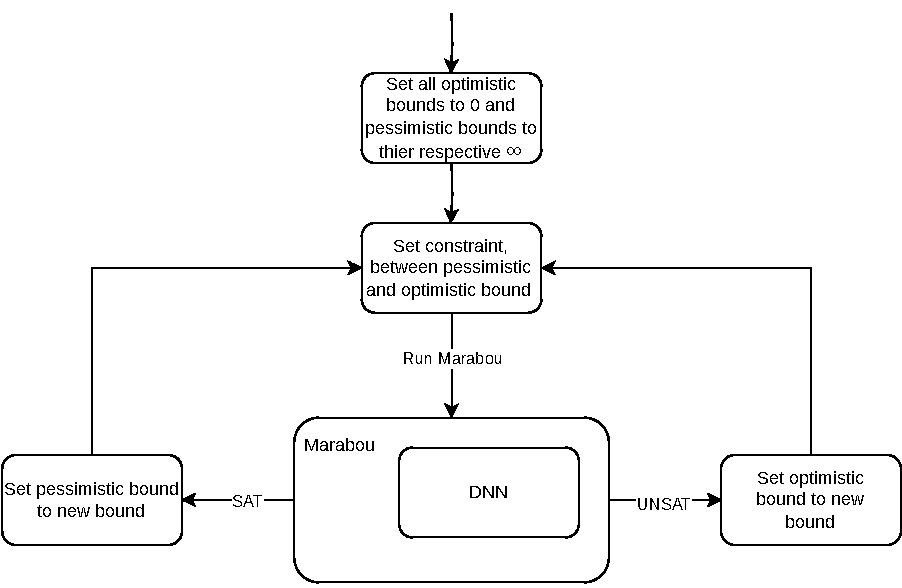
\includegraphics[width=0.75\linewidth]{figures/iterative_reluplex.pdf}
    \caption{The main loop of the Iterative Marabou, algorithm.}\label{fig:iter-marabou}
\end{figure}

The main intuition behind iterative Marabou is that increasing the optimistic bound of a variable can only every decrease the pessimistic bounds of all other problems, and never increase it. This intuition thus allows us to continuously tighten the space in which a true Pareto optimal solution lies.

To let the technique work we require that we have at least one point for which the properties hold. Finding of this point is outside the scope of this report and I instead assume this starting point to be 0. For the project I want to create an algorithm as described below: 

Algorithm \ref{alg:iter-marabou}, shows how the algorithm works. Here the algorithm is defined to take each iteration a random dimension, and then splits the search space in this dimension in two. On this bound the Marabou solver is called to check whether it upholds the constraints. If the constraints are upheld we have thus found a better pessimistic bound and can thus increase this. If the constraints are not upheld we know that there will be no bound greater than our tested bound that upholds the constraints and thus we reduce the optimistic bounds.

\begin{algorithm}[H]
\caption{Iterative Marabou algorithm}
\label{alg:iter-marabou}
\begin{algorithmic}[1]
    \State $min_{LB}[num\_input\_parameters] \gets [- \infty]$
    \State $min_{UB}[num\_input\_parameters] \gets [ 0]$
    \State $max_{LB}[num\_input\_parameters] \gets [0]$
    \State $max_{UB}[num\_input\_parameters] \gets [ \infty]$
    \item[]
    \While{$time\_to\_run > 0$}
        \State $dim \gets \text{random\_dim}()$
        \Comment{Optimize the minimum}
        \State $mid \gets (min_{LB}[dim] + min_{UB}[dim])$ \Comment{Get the midpoint as done in quickfind}
        \State $\text{addProperty}(input\_parameters[dim] \geq mid)$
        \State $upholds \gets \text{check\_properties}()$
        \If{$upholds$}
            \State $min_{LB}[dim] \gets mid$
            \Comment{If the properties still hold we found a better bound}
        \Else
            \State $\text{remove\_last\_property}()$
            \State $min_{UB} \gets mid$
            \Comment{If the properties don't hold we find a limitation of the bound}
        \EndIf
        \item[]
        \State $mid \gets (max_{LB}[dim] + max_{UB}[dim])$ 
        \Comment{Optimize the maximum}
        \State $\text{addProperty}(input\_parameters[dim] \leq mid)$
        \State $upholds \gets \text{check\_properties}()$
        \If{$upholds$}
            \State $max_{LB}[dim] \gets mid$
        \Else
            \State $\text{remove\_last\_property}()$
            \State $max_{UB} \gets mid$
        \EndIf
    \EndWhile
    \State \Return $min_{UB}, max_{LB}$
\end{algorithmic}
\end{algorithm}


\subsection*{Pareto OPtimality}
This algorithm converges to a Pareto optimal solution. This is the case because of the following two facts. The algorithm never lowers the pessimistic bound such that a feasible value would be removed from the search space, as shown in Proof \ref{proof:no-worse}. And the lowering the optimistic bound cannot result into a better pareto optimal solution. These two facts together mean that the search space of all bounds decrease every iteration, and thus eventually converges to a Pareto optimal solution.


\begin{proof}\label{proof:no-worse}
$ $
{\setlength{\parindent}{0pt}

Take $B_i^O$ for the optimistic bound for input variable $i$.

Take $B_i^P$ for the pessimistic bound for input variable $i$.

I denote $B^O$ as the set of all optimistic bounds.

And I use $B^O - B_i^O +B'$ to denote the optimistic bound set wher bound $B_i^O$ is replaced with $B'$. Finally I use $UNSAT(B)/SAT(B)$ to denote that the bounds defined by $B$ are proven to be UNSAT and SAT respectively.

We now need to proof the following:

\begin{align}
    \forall B_i' | (B_i^P < B_i' < B_i^O)\nexists B_j^P \text{ S.T. } \\
    UNSAT(B^P - B_i^P + B_i') 
    \rightarrow UNSAT(B^P - B_i^P + B_i' - B_j^O + B_j^P)
\end{align}

In other words, for all new bounds that result into an UNSAT solution it should be impossible to add a bound that previously caused the problem to be SAT to result into an UNSAT solution.

I proof this by noting that:

\begin{align}
UNSAT(B^P)
\end{align}

and

\begin{align}
\forall B_i^O SAT(B^P - B_i^P + B_i^O)
\end{align}

Thus there must be an assignment outside of the bounds of $B^P$ but inside the bounds of $B^P - B_i^P + B_i^O$. From 1 we see that the newly added bounds are always strictly higher than the old bounds, thus we get that:

\begin{align}
B^P - B_i^P + B_i^O \subset B^P - B_i^P + B_i' - B_j^O + B_j^P
\end{align}


Thus since there exist a satisfying assignment in $B^P - B_i^P + B_i^O$ there also must exists a satisfying assignment to $B^P - B_i^P + B_i' - B_j^O + B_j^P$. 
Thus we never prune a solution that is more Pareto optimal than every solution in our search space.

}
$ $
\end{proof}

\end{document}
